\section{Implementing an SDC-enabled reaction network (no diffusion)}

\subsection{Introduction to SDC}

\maestro\ integrates the following system of equations:
\begin{eqnarray}
\frac{\partial(\rho X_k)}{\partial t} &=& 
    -\nabla\cdot(\rho X_k\Ub) + \rho\omegadot_k,\label{eq:species}\\
\frac{\partial\Ub}{\partial t} &=& 
    -\Ub\cdot\nabla\Ub  - \frac{1}{\rho}\nabla\pi 
    - \frac{\rho-\rho_0}{\rho} g\eb_r,\label{eq:momentum}\\
\frac{\partial(\rho h)}{\partial t} &=& 
    -\nabla\cdot(\rho h\Ub) + \frac{Dp_0}{Dt} 
    + \rho\Hnuc ,\label{eq:enthalpy}
\end{eqnarray}
together with a constraint equation.

By default, \maestro\ uses an operator-split approach to coupling
the different physical processes together (hydro, reactions, diffusion).
With operator-splitting, we
react for a half timestep, then perform the hydrodynamics and thermal
diffusion on this intermediate state, and finally react for the
remaining half timestep to advance the solution.  For problems where
the reactions greatly alter the energy balance or composition, this
operator splitting approach can lead to inaccuracies in the solution.
This can be more of an issue for low Mach number methods that can take
large hydrodynamic time steps.

An alternate approach to coupling is spectral deferred corrections
(SDC). SDC is an iterative approach to couple the various operations
together, with each operator seeing an iteratively lagged
approximation of the other operations as a source term.  The SDC
algorithm converges to an integral representation of the solution in
time that couples all of the processes together in a self-consistent
fashion, see \cite{Non11}.

As a first attempt, we will work on coupling hydro and reactions only
via SDC, with a time-independent base state.  



\subsection{Strang-split version}

In the Strang-split version of \maestro, the reaction and advection
processes operate independent of one-another.  The species and
enthalpy equations are updated through $\Delta t$ using the following
sequence:

\begin{itemize}

\item React for $\Delta t/2$

In the Strang-split version of \maestro, the reaction network solves just
the reaction portion of the species evolution equations along with a
temperature evolution equation.  This is done using a standard ODE solver
(like {\tt VODE}) on the system:
\begin{eqnarray}
\frac{dX_k}{dt} &=& \omegadot_k(\rho,X_k,T) \\
\frac{dT}{dt}   &=& 
    \frac{1}{c_p} \left ( -\sum_k \xi_k  \omegadot_k  + \Hnuc \right ).
\end{eqnarray}
Here, $T$ is evolved solely to evaluate the reaction rates,
$\omegadot_k(\rho,X_k,T)$.  Furthermore, we simplify the problem
``freezing'' the thermodynamics---i.e., $c_p$ is evaluating at the
start of the integration and held constant thereafter.

We update the enthalpy at the end of the integration as:
\begin{equation}
h^\mathrm{new} = h^\mathrm{old} + \frac{\Delta t}{2} \Hnuc
\end{equation}

\item Advect for $\Delta t$

Here we solve
\begin{eqnarray}
\frac{\partial(\rho X_k)}{\partial t} &=& 
    -\nabla\cdot(\rho X_k\Ub) \\
\frac{\partial(\rho h)}{\partial t} &=& 
    -\nabla\cdot(\rho h\Ub) + \frac{Dp_0}{Dt} 
\end{eqnarray}

Note that no explicit reaction terms appear here.  Since the advection
takes place using the state updated from the reaction step, the effect
of the reactions is implicitly contained in the advective update.

\item React for $\Delta t/2$

Finally, we react again, starting with the state left by the advection
step.

\end{itemize}


\subsection{SDC version}
In the SDC version, the VODE integration at the end of an SDC
iteration is responsible for updating all the thermodynamic quantities
\{$\rho$, $(\rho h)$, and $(\rho X_k$)\}, including both the advective
fluxes (incorporated via a piecewise constant advective flux source
term) and the reactions.  This provides a much stronger coupling between
the physical processes.  In particular, our system now looks like:
\begin{eqnarray}
\frac{d(\rho X_k)}{dt} &=& \rho \omegadot_k(\rho,X_k,T) + A_{\rho X_k} \\
\frac{d(\rho h)}{dt}   &=& \rho \Hnuc + A_{\rho h}
\end{eqnarray}
Here, $A_{\rho X_k}$ and $A_{\rho h}$ are piecewise-constant (in time)
approximations to the change in ${\rho X_k}$ and ${\rho h}$ (respectively)
due to the advection.  These are constructed by calling {\tt density\_advance}
and {\tt enthalpy\_advance} in \maestro\ and passed into the network solver
during the reaction step.  A flowchart of the \maestro\ SDC algorithm is 
shown in figure~\ref{fig:sdc:flowchart}.

\begin{figure}[tb]
\centering
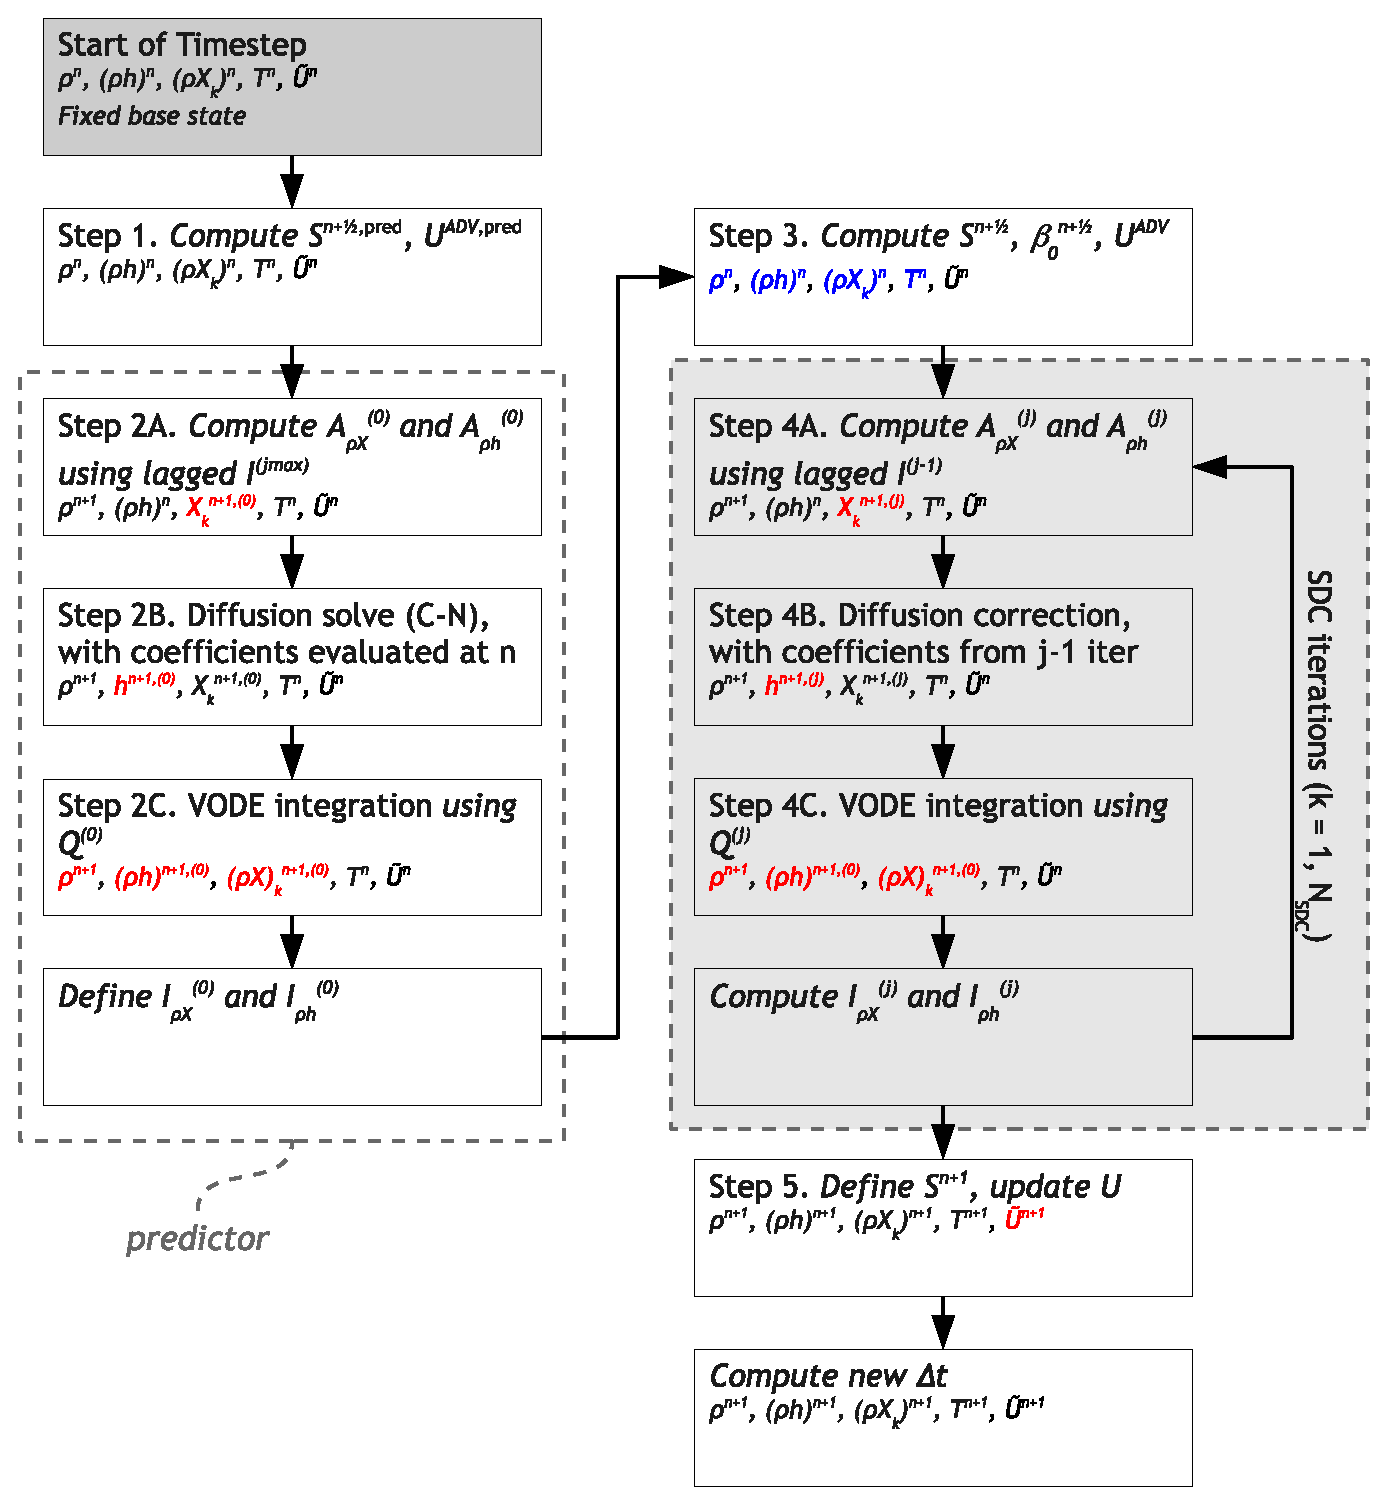
\includegraphics[scale=0.65]{\sdcfigpath/flowchart_SDC}
\caption[Graphical flowchart of \maestro\ SDC]
  {\label{fig:sdc:flowchart} A flowchart of the \maestro\ SDC algorithm.  The
  thermodynamic state variables and local velocity are
  indicated in each step.  The base state is not shown as it is time-independent.
  Red text indicates that quantity was
  updated during that step.  The predictor is 
  outlined by the dotted box.  The blue text indicates state
  variables that are the same in {\bf Step 6} as they are in
  {\bf Step 2}, i.e., they are unchanged by the predictor steps.
  The SDC loop is shown in the gray dotted box.}
\end{figure}


\subsubsection{Advective Update}

In the advective update, our goal is to compute $A_{\rho X_k}$ and
$A_{\rho h}$.  These terms approximate the following:
\begin{eqnarray}
A_{\rho X_k} &=&  \left [- \nabla \cdot (\rho X_k \Ub) \right ]^{n+1/2} \\
A_{\rho h}   &=&  \left [- \nabla \cdot (\rho h U) + \frac{Dp_0}{Dt} \right ]^{n+1/2}
\end{eqnarray}
The construction of the interface states used in the advective terms
uses an iteratively-lagged approximation to the reaction source terms
($I_{\rho X_k}$ and $I_{\rho h}$, see below) in the interface
prediction.  This explicitly couples the reaction process to the
advection process.


\subsubsection{Final Update}

The RHS routine that the ODE solver operates on will first construct
the density as:
\begin{equation}
\rho = \sum_k (\rho X_k)
\end{equation}
It will then derive the temperature from the equation of state.  If we
are running with {\tt use\_tfromp = T}, then we do
\begin{equation}
T = T(\rho, p_0, X_k)
\end{equation}
otherwise, we do
\begin{equation}
T = T(\rho, h, X_k)
\end{equation}
Note that in constrast to the Strang-split version, here we call the EOS
every time we enter the RHS routine.

At the end of the integration, we define $I_{\rho X_k}$ and $I_{\rho
  h}$.  The actual form of these depends on what we are predicting.
We note that we only need $I_{\rho X_k}$ and $I_{\rho h}$ for the
prediction of the interface states, not the final conservative update.
That is because all we need from the advection solver is the
approximation to $A_{\rho X_k}$ and $A_{\rho h}$, not the final
updated state.

\paragraph{Species Source Terms.}
For the species prediction, the form of $I_{\rho X_k}$ depends on
{\tt species\_pred\_type} (see \S \ref{sec:pred:density}):  
\begin{itemize}
\item {\tt species\_pred\_type} = 1 (predict $\rho'$ and $X_k$)
%
\begin{equation}
I_{\rho X_k} = \frac{1}{\rho^{n+\myhalf}} \left [ 
      \frac{(\rho X_k)^\mathrm{new} - 
            (\rho X_k)^\mathrm{old}}{\Delta t} - A_{\rho X_k}  \right ]
\end{equation}

\item {\tt species\_pred\_type} = 2 (predict $\rho'$ and $(\rho X_k)$)
%
\begin{equation}
I_{\rho X_k} = \frac{(\rho X_k)^\mathrm{new} - (\rho X_k)^\mathrm{old}}{\Delta t} - A_{\rho X_k} 
\end{equation}

\item {\tt species\_pred\_type} = 3 (predict $\rho$ and $X_k$)
%
\begin{equation}
I_{\rho X_k} = \frac{1}{\rho^{n+\myhalf}} \left [ 
      \frac{(\rho X_k)^\mathrm{new} - 
            (\rho X_k)^\mathrm{old}}{\Delta t} - A_{\rho X_k}  \right ]
\end{equation}

\end{itemize}

We note that there is no $I$ term for $\rho$ or $\rho'$ prediction, since
the density evolution equation does not have a reaction source term.

\paragraph{Enthalpy Source Terms.}
For the enthalpy prediction, the form of $I_{\rho h}$ depends on
{\tt enthalpy\_pred\_type} (see \S \ref{sec:pred:enthalpy}).:
\begin{itemize}
\item {\tt enthalpy\_pred\_type} = 1 \\
not right -- should be pert form
if we do something in perturbational form, then don't we need to have
the base state see the reaction term in its prediction?
\begin{equation}
I_{\rho h}  = \frac{(\rho h)^\mathrm{new} - (\rho h)^\mathrm{old}}{\Delta t} - A_{\rho h}
\end{equation}
\end{itemize}


\ \\
This is done in {\tt advance.f90} just after the call to {\tt react\_state},
stored in the \multifab\ called {\tt intra}.
These terms are used as the source terms for the
advection step in the next SDC iteration.

\subsection{Summary of Changes}
The major changes from the non-SDC-enabled burners is the addition of
the advective terms to the system of ODEs, the fact that we integrate
$(\rho X_k)$ instead of just $X_k$, and the need to derive the
temperature from the input state for each RHS evaluation by {\tt
  VODE}.

Note also that the SDC integration by {\tt VODE} does not operate on 
the velocities at all.  That update is handled in the same fashion 
as the Strang-split version of the code.

The {\tt ignition\_simple\_SDC} burner shows how to setup the system
for {\tt use\_tfromp = T} or {\tt F}.  Presently, this implementation
does not support {\tt evolve\_base\_state = T} (in particular, we 
need to evolve $p_0$ in the RHS routine).
